% !TeX root = ../thuthesis-example.tex

\chapter{卷积神经网络分层抽象特性和遗忘方法}
上一章阐述了遗忘学习的研究现状以及相关研究工作。本章首先介绍卷积神经网络的一个重要特性,分层抽象特性。为了让读者能够更好地理解卷积神经网络的分层抽象特性,首先将介绍卷积神经网络的工作原理以及设计思想。
接下来介绍卷积神经网络分层抽象特性和遗忘方法。最后介绍评价遗忘效果的性能指标。

\section{卷积神经网络介绍}

\subsection{卷积神经网络结构}

\begin{algorithm}  
    \caption{用归并排序求逆序数}  
    \begin{algorithmic}[1] %每行显示行号  
        \Require $Array$数组,$n$数组大小  
        \Ensure 逆序数  
        \Function {MergerSort}{$Array, left, right$}  
            \State $result \gets 0$  
            \If {$left < right$}  
                \State $middle \gets (left + right) / 2$  
                \State $result \gets result +$ \Call{MergerSort}{$Array, left, middle$}  
                \State $result \gets result +$ \Call{MergerSort}{$Array, middle, right$}  
                \State $result \gets result +$ \Call{Merger}{$Array,left,middle,right$}  
            \EndIf  
            \State \Return{$result$}  
        \EndFunction  
        \State  
        \Function{Merger}{$Array, left, middle, right$}  
            \State $i\gets left$  
            \State $j\gets middle$  
            \State $k\gets 0$  
            \State $result \gets 0$  
            \While{$i<middle$ \textbf{and} $j<right$}  
                \If{$Array[i]<Array[j]$}  
                    \State $B[k++]\gets Array[i++]$  
                \Else  
                    \State $B[k++] \gets Array[j++]$  
                    \State $result \gets result + (middle - i)$  
                \EndIf  
            \EndWhile  
            \While{$i<middle$}  
                \State $B[k++] \gets Array[i++]$  
            \EndWhile  
            \While{$j<right$}  
                \State $B[k++] \gets Array[j++]$  
            \EndWhile  
            \For{$i = 0 \to k-1$}  
                \State $Array[left + i] \gets B[i]$  
            \EndFor  
            \State \Return{$result$}  
        \EndFunction  
    \end{algorithmic}  
\end{algorithm}  


卷积神经网络和多层感知机的神经网络类似,它们都可以通过像堆积木一样来组装构建。卷积神经网络和多层感知机不同的是卷积网络特有的卷积层(Convolution Layer)和池化层(Pooling Layer)。

% 基于多层感知机的神经网络中,相邻层的各个神经元之间都有连接,这样的结构被称为全连接(Fully-Connected)。
% 如果使用全连接层来搭建网络,我们可以通过如图\ref{fig:chapter3_3}所示的神经网络结构实现一个五层的简单神经网络。
% 如图\ref{fig:chapter3_3}所示,在使用全连接层搭建的神经网络中,全连接层后面直接跟着激活函数ReLU(或者Sigmoid)。这里使用了4 层全连接和ReLU的组合,接着的第5层是全连接层,最后一层则是Softmax层,输出最终的预测结果。
% \begin{figure}
%     \centering
%     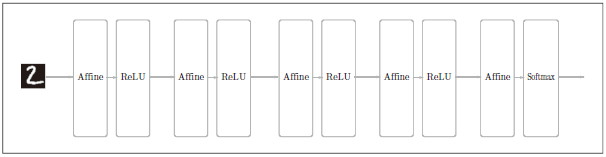
\includegraphics[width=0.9\linewidth]{chapter3_3.png}
%     \caption{全连接网络结构示意图\cite{luyujie_216}}
%     \label{fig:chapter3_3}
% \end{figure}
\begin{figure}
    \centering
    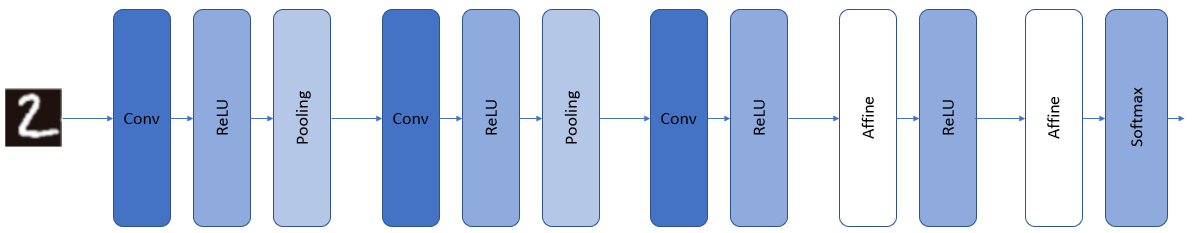
\includegraphics[width=0.9\linewidth]{chapter3_2.png}
    \caption{卷积神经网络结构示意图}
    \label{fig:chapter3_2}
\end{figure}

如图\ref{fig:chapter3_2}所示,这是一个卷积神经网络的例子。卷积神经网络的单个层连接的顺序是卷积层、激活函数层(如图中的ReLU层)和池化层,其中池化层有时可以省略。
然后,最终的输出层中则使用了全连接层和Softmax的组合。图中的Affine层代表全连接层。这样的搭配一般都是卷积神经网络中较为常见的搭配结构。
卷积层主要用来提取特征,激活函数层主要用来过滤卷积层提取到的特征,对输入的特征增加非线性的因素,因为线性模型的表达能力是有限的。池化层主要用来压缩数据和参数的量,因此也常被称为下采样层。
全连接层能够实现特征的空间映射,常被用来做分类器。Softmax层是对整个网络输出结果的优化表示,将神经网络的输出转换成概率分布的输出,以便于对网络输出的理解。

\subsection{卷积神经网络原理} 
\subsubsection{卷积神经网络对于位置关系的理解}
在全连接的神经网络中,每一层都是通过全连接层组织起来的。在全连接的层次中,各个神经元都是连接在一起的,其输出数量是可以任意指定的,没有数量上的限制。

这样的结构没有将数据的形状特征充分利用起来。用图片来举例,神经网络输入图片时,图片数据的格式一般是长、宽和高。长和宽代表图片以像素为单位的长度和宽度,高代表图片采样通道的宽度。
然而,这样的数据结构输入到全连接层搭建的神经网络中时,就会被展开成一维的数据。图片一般是三维的形状,即图片的长度和宽度,还有色彩的维度(红色通道,绿色通道,蓝色通道),这样的形状结构中包含了重要的空间位置关系信息。
比如色彩通道之间的关联信息,空间上相互距离比较接近的像素点一般具有相似的值,距离比较远的像素点一般没有关联。因此三维形状的数据中可能会蕴藏很多可以挖掘的特征模式。全是全连接层的神经网络就会把数据展开成一维数据,从而没有充分利用图片中的空间位置信息。
卷积神经网络会将图片以三维数据的格式输入到网络中,一个卷积层处理好数据以后,仍然会以三维的数据格式输入到下一个卷积层中。所以,卷积神经网络对于理解带有空间位置信息的数据具有一定的优势。

\subsubsection{卷积层}
卷积运算发生在卷积层,卷积运算的计算过程类似滤波处理的过程。因此用于卷积运算的卷积核有时又被称为滤波器。常规的卷积运算如图\ref{fig:chapter3_4}所示。
图中展示了一次二维卷积运算的运算过程。输入数据的尺寸是4乘4,卷积核的尺寸是3乘3,在没有边界填充并且步长为1的情况下,最终输出结果的尺寸是2乘2。
\begin{figure}
    \centering
    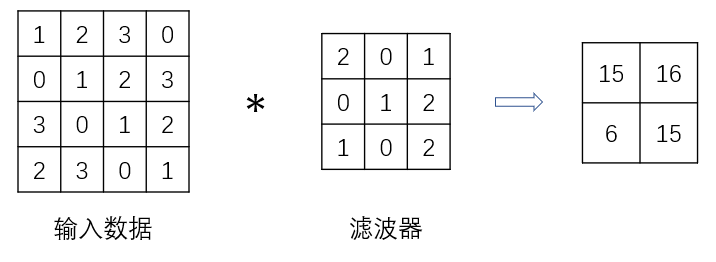
\includegraphics[width=0.6\linewidth]{chapter3_4.png}
    \caption{卷积运算后数据大小发生变化}
    \label{fig:chapter3_4}
\end{figure}

图\ref{fig:chapter3_5}中介绍了卷积运算的完整过程。图中第一行灰色区域代表第一步卷积操作所发生的区域,这个区域内的数字和卷积核的形状是相同的,所以区域内的数字可以与卷积核中对应位置的数字相乘,然后再把这些相乘的结果相加就得到了第一个结果。
运算后将结果保存到相应的位置。在图\ref{fig:chapter3_5}中第二、三、四行将上述过程在每个位置计算一遍,就完成了输入数据在一个卷积核上的特征输出。
\begin{figure}
    \centering
    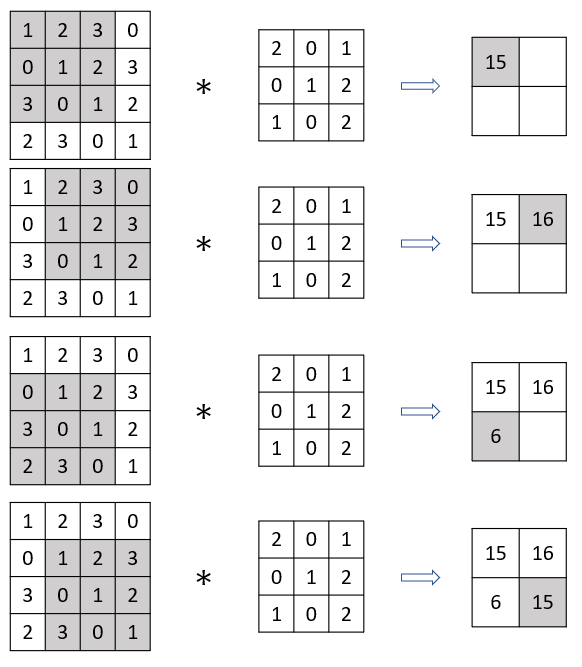
\includegraphics[width=0.5\linewidth]{chapter3_5.png}
    \caption{卷积运算过程示意图}
    \label{fig:chapter3_5}
\end{figure}

卷积神经网络中除了权重之外,还有偏置。卷积神经网络中偏置的个数一般就是卷积核的个数,而且每个卷积核对应的偏置维度一般是1乘1。
计算完卷积之后,在相应结果的每个位置再加上偏置数字便得到了最终输出的数据,其计算过程如图\ref{fig:chapter3_6}所示。
对于输入数据,滤波器与输入数据进行卷积运算后便得到了初步的输出结果。之后再将这个结果的每一个位置加上该卷积核对应的偏置数值,得到了最终结果。
\begin{figure}
    \centering
    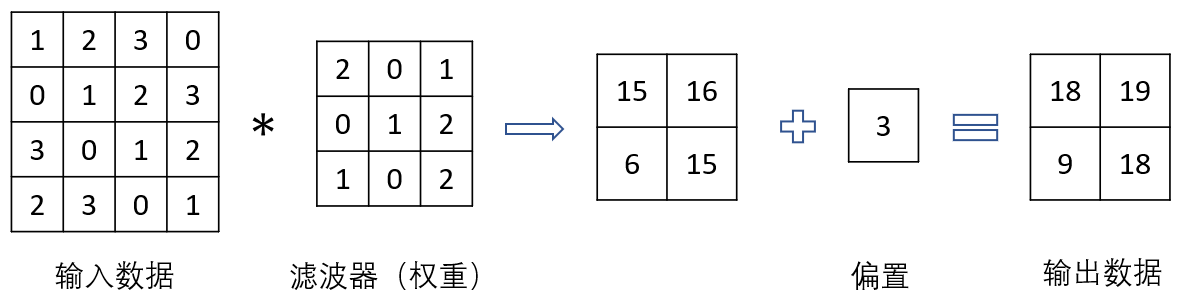
\includegraphics[width=0.7\linewidth]{chapter3_6.png}
    \caption{卷积运算后的偏置}
    \label{fig:chapter3_6}
\end{figure}

三维卷积运算与二维卷积运算不同的是,卷积核的维度从二维提高到了三维,除了有长和宽的信息,还有通道的维度。以三通道为例,其运算过程与二维相似,先将对应位置的数字相乘,然后将相乘之后的结果相加,便得到了输出结果。

\subsubsection{池化层}
为了减少参数的数量,提高神经网络泛化能力,在卷积神经网络进行卷积运算以后,通常会进行池化操作。池化操作会同时减少卷积操作结果的长度和宽度。
其运算过程如图\ref{fig:chapter3_8}所示。在图中第一行,灰色区域就是池化的一个操作单元。这个操作单元的大小来自池化操作的输入参数。
池化操作的输入是图中灰色区域内的数字,输出是一个数字。中间的运算过程一般有两个算法,一种是取所有数字中最大的数字,这种算法被称为最大池化操作;另外一种算法是取区域内所有数字的平均数,这种算法被称为平均池化操作。
\begin{figure}
    \centering
    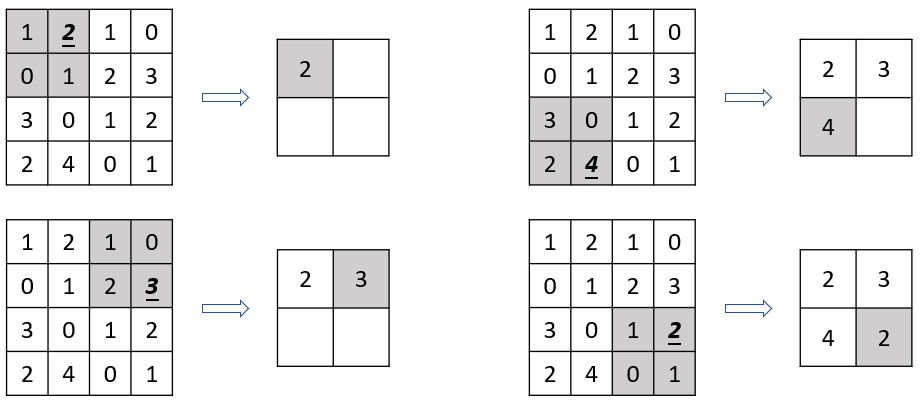
\includegraphics[width=0.7\linewidth]{chapter3_8.png}
    \caption{池化操作流程图}
    \label{fig:chapter3_8}
\end{figure}

池化层与卷积层不一样的是,池化层没有训练参数,它的输入参数都是运算之前系统已经规定好的超参数。池化层就是一个固定算法的函数。它另外的一个特点是,池化操作后通道数是不变的,各通道是相互独立的。
加入池化层后,神经网络对输入数据存在的微小干扰具有很好的鲁棒性。如图\ref{fig:chapter3_10}所示,即使图片向右发生了1个偏移,经过池化操作后,其特征仍能被准确地识别出来。
\begin{figure}
    \centering
    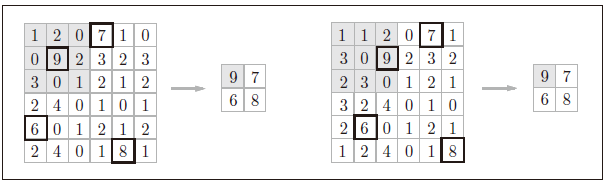
\includegraphics[width=0.9\linewidth]{chapter3_10.png}
    \caption{池化操作对发生偏移的输入具有鲁棒性}
    \label{fig:chapter3_10}
\end{figure}

\section{卷积神经网络分层抽象特性}
为了更好地理解卷积神经网络的分层抽象特性,我们首先简要地介绍生物视觉信息处理的原理。
\subsection{生物视觉系统对信息的分层处理}
1981年来自美国的科学家David Hunter Hubel和来自瑞典的科学家Torsten Wiesel被授予了诺贝尔生理学或医学奖,以表彰他们在探究人类视觉系统信息加工过程中做出的杰出贡献\cite{Hubel1998EarlyEO}。他们的工作成为了所有研究神经生物学学生们的必学内容。
他们使用探针记录了麻醉后猫的大脑视觉皮层神经元的活动\cite{https://doi.org/10.1113/jphysiol.1959.sp006308}。
他们在实验中发现,有一类细胞对一定视野范围内特定朝向上移动的狭长光斑反应强烈,而且反应的产生有明显的边界。方向不对或者超越边界都无法使之产生反应。
当光斑覆盖整个作用区域时,也无法产生刺激反应。这样的细胞被看作是用来感受线条或边缘信号的接收器。后来他们将这样的现象称为神经细胞的朝向选择性,称这样的神经细胞为简单细胞。
他们通过进一步的实验发现,还有一类细胞虽然对特定方向光斑的刺激有强烈反应,但是并没有明显的感受边界。他们发现这样的细胞上游是许多的简单细胞,而且刺激信号均是来自这些简单细胞。
他们称这些具有朝向选择性,但是没有明显的反应边界的细胞为复杂细胞。这一发现初步揭示了猫的视觉系统信息处理具有分层的特点。

\subsection{分层抽象特性}
LeCun\cite{726791}提到过卷积神经网络的设计思想参考了生物视觉信息处理中简单细胞和复杂细胞\cite{hubel1962}的概念。
Kubilius Jonas等人\cite{2019arXiv190906161K}提到了卷积神经网络是最接近还原人类视觉信息加工原理的人工神经网络。在卷积神经网络中,层数较低的卷积核提取的是较为初级的基本特征,层数较高的卷积核提取的特征是比较抽象的特征。
随着输入数据在多层卷积层中逐层传递,一些特征信息逐渐被卷积核提取,提取的信息也逐步抽象。本文将卷积神经网络这种区别于其他人工神经网络的特性称为卷积神经网络的分层抽象特性。
如图\ref{fig:chapter3_13}所示, 图中上半部分展示了一个训练完成的AlexNet\cite{alexnet2017}的8层卷积神经网络结构,下半部分则是参数可视化\cite{Zeiler2014,Mahendran_2015_CVPR}后的效果。
我们可以看到第一个卷积层学到的信息是一些基础的信息,例如边和角;第三层学到了由边和角构成的类似材质的图案;第五层则学到了由图案构成的物体的某个部分;最后,全连接层学到的是整个物体本身。
由此可以看出在卷积神经网络模型中,越靠后面的层次提取的特征越抽象(这里我们称离输入端较近的层次为前面层次,离输出端较近的层次为后面层次),这种现象就解释了我们所说的分层抽象特性。
\begin{figure}
    \centering
    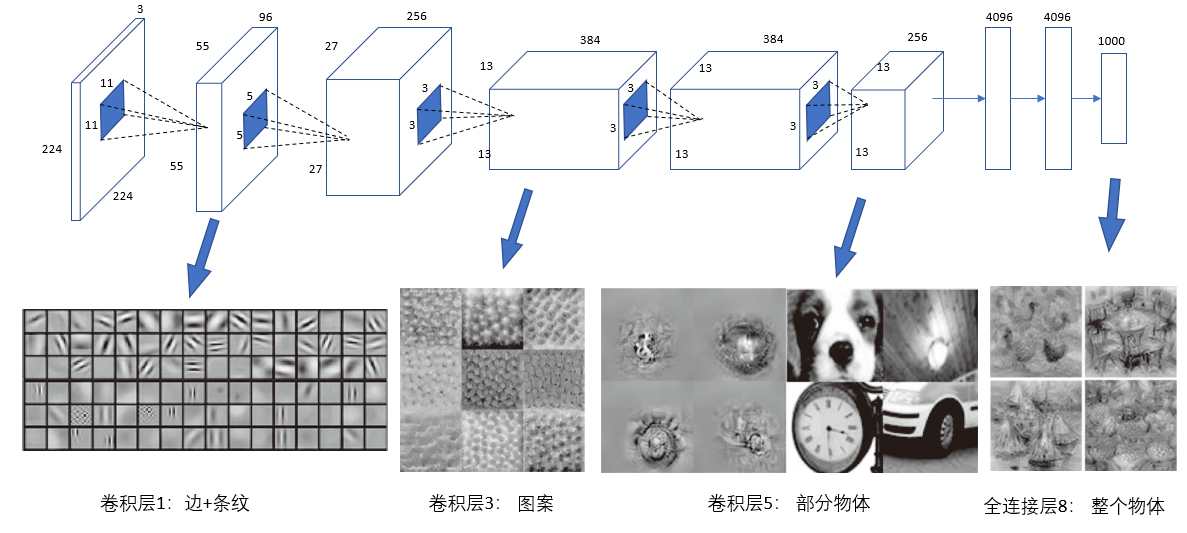
\includegraphics[width=0.9\linewidth]{chapter3_13.png}
    \caption{卷积神经网络的分层抽象特性示意图}
    \label{fig:chapter3_13}
\end{figure}


我们用一个手写两层卷积运算过程的例子来举例说明这种抽象特性。
如图\ref{fig:chapter3_15}所示,图中分为上下两个部分,这两个部分使用两个相同卷积核进行卷积运算,输入数据为图片最左端的的矩阵。$\ast$符号代表卷积运算。将两个卷积运算的结果相加得到了第一卷积层的输出结果。
下面一层也是如此,输入数据经过与两个卷积核运算以后,将运算结果相加,便得到了第一卷积层的输出结果。经过仔细观察后,这张图片的两个卷积核具有明显的特征,上面的卷积核用于提取主对角线的特征,下面的卷积核主要提取次对角线的特征。这些都是较为基本的特征。
经过两个卷积核特征提取后,再将计算结果相加,就得到了两个卷积核特征的相加结果。
\begin{figure}
    \centering
    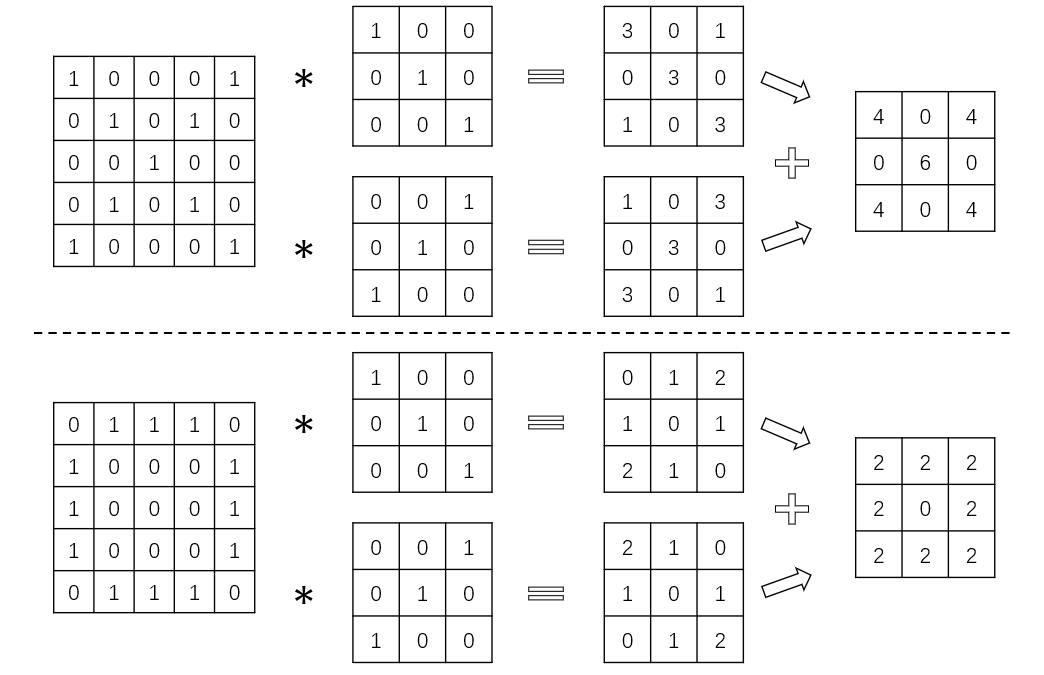
\includegraphics[width=0.9\linewidth]{chapter3_15.png}
    \caption{手写卷积运算示意图1}
    \label{fig:chapter3_15}
\end{figure}

将图\ref{fig:chapter3_15}的输出结果分别再使用两个卷积核进行卷积运算。运算之后分别得到两个运算结果,如图\ref{fig:chapter3_16}所示。
左右两图中分别有两个卷积核,这两个卷积核是对应相等的。仔细观察后可以发现,上面的卷积核主要提取的特征是X形特征的信息;而下面的卷积核主要用于提取O形特征的信息。
图\ref{fig:chapter3_16}(a)中两个卷积运算的结果分别是22和10,这说明图\ref{fig:chapter3_15}上面的输入图片相比于下面的图片更像X形。图\ref{fig:chapter3_16}(b)中两个卷积运算的结果分别是8和16。
这说明图\ref{fig:chapter3_15}下面的输入图片相比于上面的图片更像O形。
相似的结论我们通过肉眼比较也可以得出。通过此例可以明显地感觉到较高层次卷积核的感受野比低层次卷积核的感受野更大。第一卷积层卷积核的感受野是3乘3的方形区域,第二卷积层的感受野是整张图片,即5乘5的方形区域。
由此可见,较高层次的卷积核往往更加关注提取较为抽象的信息,较低层次的卷积核更加关注提取较为基本的信息。
\begin{figure}
    \centering
    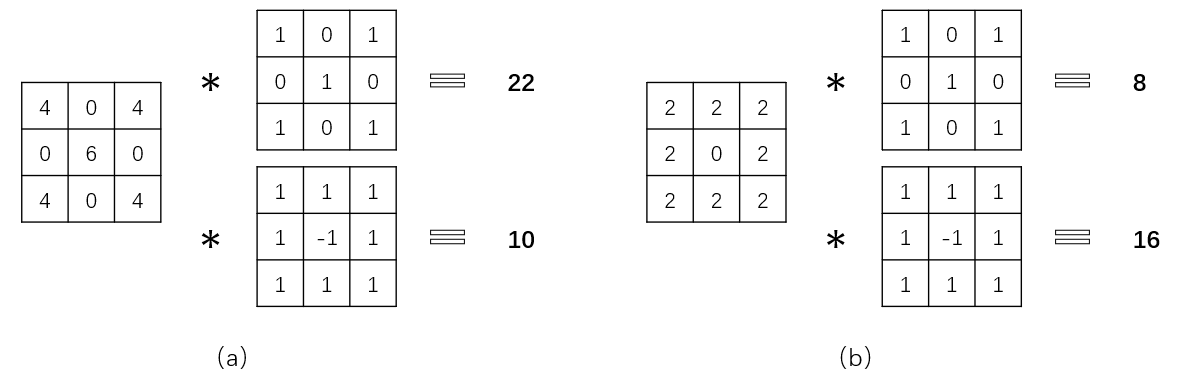
\includegraphics[width=1\linewidth]{chapter3_16.png}
    \caption{手写卷积运算示意图2}
    \label{fig:chapter3_16}
\end{figure}

\section{卷积神经网络遗忘方法介绍}
本节首先介绍遗忘方法的基本思路,然后再讨论遗忘方法的具体步骤。
\subsection{遗忘方法思路}
对一个已经使用数据训练过的神经网络而言,其理想的遗忘效果是,就好像这个神经网络模型从来没有使用要遗忘的数据训练过一样。对于一个用户来说,他不希望自己的数据能够被攻击者窃取或被还原。
当前针对神经网络的攻击方法多种多样,我们与其针对每种攻击方法去设置防御方案,倒不如直接遗忘神经网络模型中指定数据的信息。我们遗忘的信息越多,攻击者得到的信息就越少。遗忘信息的完美情况就是重新训练。
然而重新训练的代价是十分巨大的,一个神经网络模型少则几千个参数,多则高达数亿参数,重新训练的代价是十分昂贵的。所以完全遗忘所有信息看起来是不现实的,我们能做的是尽可能地接近完美情况。
受到卷积神经网络分层抽象特性的启发,我们可以仅遗忘较为抽象的信息,保留一些基本的信息。就像人类视觉信息处理过程一样,卷积神经网络较低层次的卷积层只提取了较为基本的视觉元素,比如边、角、简单的条纹等等。
随着网络层次的提高,抽象程度逐渐提高,比如提取到一些有固定模式的组织,图案等。到卷积神经网络比较高的层次后,卷积核能提取到跟分类息息相关的本质特征,比如不同人脸的区分,以及不同物体的区分,例如猫和狗,飞机和卡车等。
一些基本的特征即使不用窃取,攻击者也能通过类似的模型训练中还原出来。所以攻击者最想获取到的是和分类有关的本质特征信息,而不是基本特征信息。
我们利用这个思路想出了一个既可以遗忘信息,又能不用训练全部参数的折中方案:重置卷积神经网络中靠近输出若干层次的网络参数,再用没有被遗忘的训练集去训练模型,直至模型收敛,同时在训练过程中保持参数没有被重置的层次始终处在冻结状态。
具体过程如图\ref{fig:chapter3_14}所示。
\begin{figure}
    \centering
    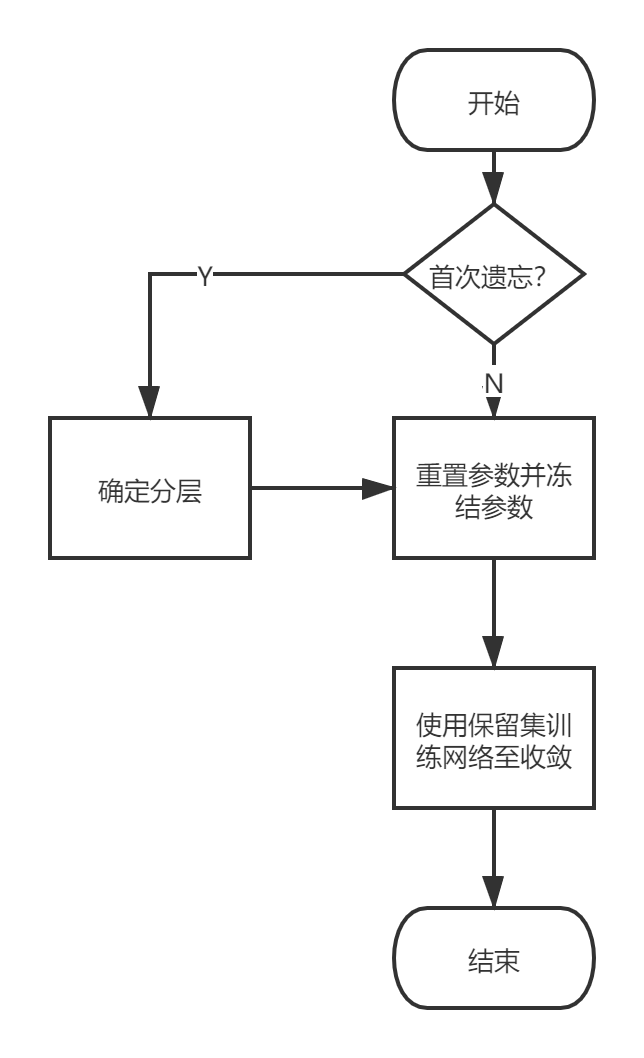
\includegraphics[scale=0.25]{chapter3_14.png}
    \caption{遗忘方法流程图}
    \label{fig:chapter3_14}
\end{figure}

本文主要讲遗忘方法,因此为了表述方便,我们定义需要遗忘的训练数据集为遗忘训练集,原来的训练数据集除去遗忘训练集后称为保留训练集。与数据集的定义类似,在本文我们称要遗忘的类别为遗忘类别,所有类别除去遗忘类别称为保留类别。
测试集中标签是遗忘类别的测试数据组成的集合称为遗忘测试集,由标签是保留类别所组成的测试数据集称为保留测试集。

\subsection{确定分层}
确定如何分层是本方法的一个重要环节,因为重置层数的多少直接影响了遗忘效果的好坏以及重新训练的时间。为了确定分层,我们分两个步骤来进行:第一步是分层预选,第二步是分层评估,下面将分别介绍。

分层的第一步是分层预选,其目的是先找出可能适合分层的层次,排除掉不适合分层的层次。具体方法是通过反向重置冻结参数训练的方法来寻找预选分层。
如图\ref{fig:chapter3_reverse_freeze_1}所示,仍然以8层的AlexNet网络为例。卷积神经网络训练好以后,将其参数分成前后两个部分,分开的方法是从离输入层最近的层次开始分起,离输入层最近的层次作为前面层次,其余所有层次作为后面层次。
\begin{figure}
    \centering
    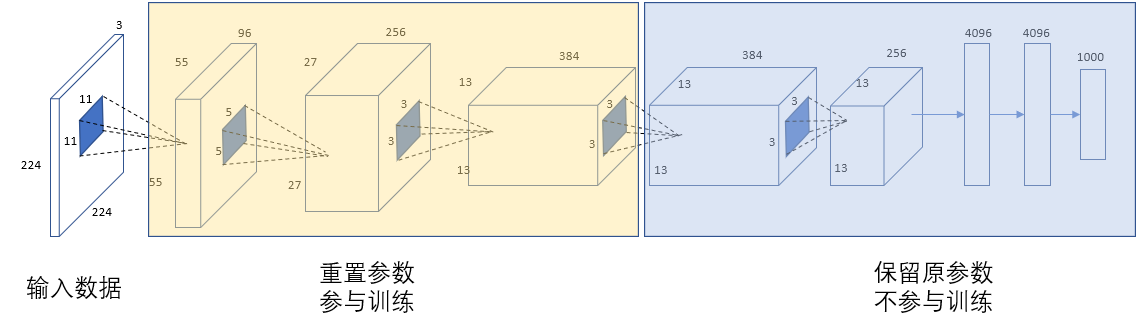
\includegraphics[scale=0.4]{chapter3_reverse_freeze_1.png}
    \caption{反向重置冻结训练方法示意图}
    \label{fig:chapter3_reverse_freeze_1}
\end{figure}
然后,将前面层次的参数初始化成该网络训练之前的对应层次的参数,后面的层次仍然保留原有的参数不变。
最后,将原来的数据集分成两个部分,第一部分仅包含遗忘类别的训练数据,第二部分仅包含保留类别的训练数据。然后用仅包含保留类别的训练数据重新训练网络,直到网络收敛为止,保存训练后的参数。在训练过程中保持只训练前面的参数,后面的参数不参与训练。
经过上述步骤以后,我们再将离输入层较近的两层作为前面的层次,其余层次作为后面的层次。再进行上述步骤,直到网络收敛并保存训练后的参数。以此类推,直到前面参数为全部的参数为止,此时后面的参数为空。
经过上述过程之后,我们将得到和网络层数相同的训练好的模型。然后分别测量这些网络在遗忘测试数据集上的准确率,然后绘制准确率曲线。绘制的准确率曲线大致趋势如图\ref{fig:chapter3_reverse_freeze_2}所示。
\begin{figure}
    \centering
    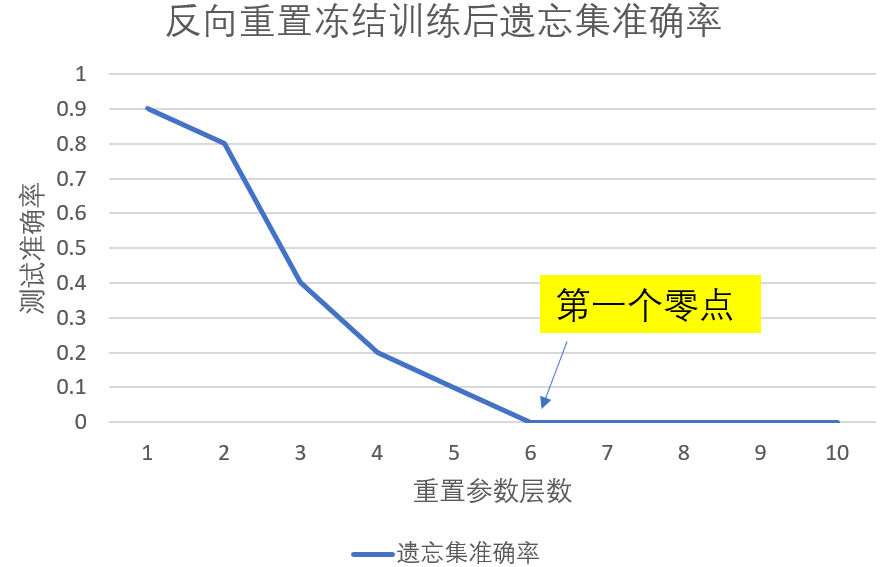
\includegraphics[scale=0.4]{chapter3_reverse_freeze_2.png}
    \caption{反向重置冻结训练后遗忘准确率曲线}
    \label{fig:chapter3_reverse_freeze_2}
\end{figure}
图中展示了反向重置训练后遗忘测试集准确率的大致曲线。重置参数层数较少时,遗忘集测试准确率仍然有较高的数值,说明需要遗忘的数据并没有被遗忘。直到某个点接近零后,后面所有的层次全部为零。我们称第一个近似为零的点为“第一个零点”。
这也是我们预选分层的地方。我们将“第一个零点”的位置作为我们确定分层的预选位置。于是,我们就完成了确定分层的第一个步骤。

预选分层以后,我们仍然不能确定实施该分层后的遗忘效果。为了更好地确定分层,我们进行确定分层的第二个步骤,分层评估。其具体做法是通过正向重置冻结训练的方法测试各个层次的评价指标,然后综合这些评价指标来最终确定分层。
正向重置冻结参数训练的方法如图\ref{fig:chapter3_reset_freeze}所示。首先,将网络参数分成前后两个部分。分开的方法仍然是逐层进行。
第一次先将离输出层最近的一层作为后面层次,其余层次作为前面层次。第二次将离输出层最近的两层作为后面层次,其余层次作为前面层次。以此类推,直到所有层次均作为后面层次,前面层次为空为止。
然后,将后面的层次初始化,将前面的层次保持原有状态不动。
最后,将原来的数据集分成两个部分,第一部分仅包含遗忘类别的数据,第二部分仅包含保留类别的数据。使用仅包含保留类别的数据去训练重置参数后的模型,直到模型收敛为止。在训练过程中,保持前面层数保持冻结,不参与参数更新过程。
\begin{figure}
    \centering
    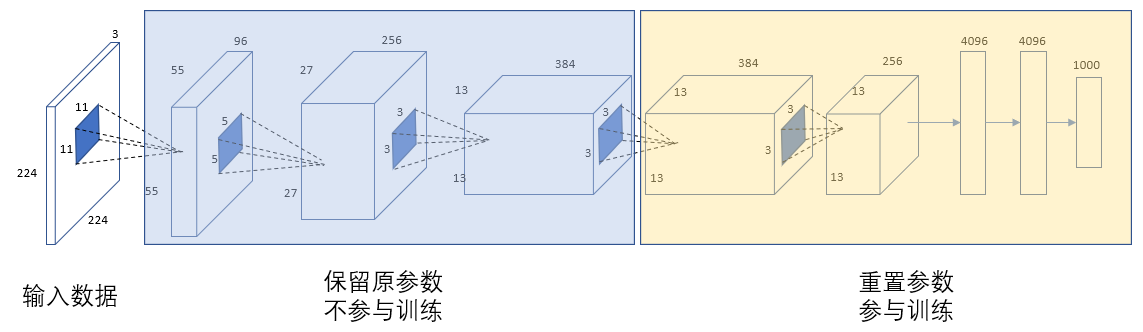
\includegraphics[scale=0.4]{chapter3_reset_freeze.png}
    \caption{正向重置冻结训练方法示意图}
    \label{fig:chapter3_reset_freeze}
\end{figure}
训练好模型后,我们将得到和参数层数数量相同的模型。分别测试这些模型的相应指标:首先是准确率。准确率分为两大类,一类是只使用遗忘数据集测试的遗忘测试准确率,另一类则是只使用保留数据集测得的保留测试准确率。
选择这个指标是出于实际应用的考虑。因为我们训练神经网络模型的目的是用于分类,所以一个最基本的要求就是要在保留的数据集上有较高的分类准确率,在遗忘的数据集上要有和重新训练的模型类似的准确率。
其次是重新训练时间,这也是十分重要的指标。重新训练时间如果长于完全重新训练的时间,那么本方法就没有了存在的价值。
有了上述确定分层的指标,我们就可以对分层结果进行评价。具体的评价原则是:首先,尽可能地接近预选层数。其次,对于遗忘类别准确率尽可能为0,对于保留类别准确率尽可能地高。对于收敛时间,要尽可能地低。
尽可能地接近预选层数是为了保证遗忘的效果。因为通过实验我们发现虽然重置较后面的层次能够达到较高的保留准确率和较低的遗忘准确率和较快的收敛时间,但是并不能保证激活距离与完全重新训练保持足够的接近。
实验数据表明,重置参数层数越多,激活距离越接近。预选层数可以满足这一要求,通过预选层数,我们可以知道到了哪一层才与最终的分类直接相关。尽可能地接近预选层数,也就是要尽可能多地重置与分类相关的层次。
再有,通过考虑遗忘准确率、保留准确率还有收敛时间,我们可以保证遗忘后的使用效果和训练过程时间的可控。

需要说明的一点是,在本方法中我们无需在每次遗忘时均确定分层,仅需在首次使用时确定分层。实验结果表明,确定一次分层可以很好地支持神经网络进行连续的遗忘操作。
在实际寻找预选层次过程中,我们无需对网络的每一个层次均进行测试,可以使用二分查找的方法来加速查找过程。
比如使用一个层数为10层的卷积神经网络时,假设“第一次零点”是从输入层开始的第四层。我们可以先查找第5层,因为第5层的遗忘准确率为0,我们再利用一次二分查找,这次是第3层。
结果发现第3层的遗忘集准确率不为0,再利用一次二分查找,这次是第4层。当我们发现第4层的遗忘测试准确率为0时,我们就能确定预选层数是第4层,这可以使得预选层数的查找算法复杂度从$O(n)$降到$O(\log n)$。

\subsection{重置并冻结参数}
确定好如何分层后,就要重置从分层点开始到输出层的所有参数,并且将没有被重置的参数冻结,防止在训练中被更新。重置并冻结参数的原因是为了减少遗忘数据在原网络中的信息,并且保留和分类关系不密切的基本信息。
对于重置和冻结参数,我们将分开进行解释。

重置参数就是将一些层次的参数使用另外一些数值代替。如果替代的参数选择不当,可能会导致模型无法收敛,或导致无法达到全局最优等问题。
为了防止这样的由于参数初始化不当而带来的问题,我们选取的策略是,保存模型的初始化参数。当网络中某些层次需要重置参数时,我们将保存下来的相应层次最初的网络参数补充到需要重置参数的层次当中。
这样做的原因是,既然这个网络模型初始化参数能够使得网络达到收敛状态,就说明这个参数是一个较为合理的初始化参数,没有均值过大或过小,方差过大或过小的异常情况。
经过实验证明,这种做法能够达到理想的效果,在实验中并未发现由于重置参数不当而带来的网络训练无法收敛的问题。

对于冻结网络,需要关注的问题是冻结网络的必要性。为了探究是否有必要冻结参数,本文设计了冻结参数与非冻结参数的对比实验,实验过程和结果将在下一章中展示。

\subsection{训练网络}
重置并冻结参数后,我们要使用保留集继续训练被重置的参数,直至网络再次收敛。再次训练网络时,使用的数据集是保留训练集。
重新训练网络的目的是为了还原保留类别的信息。因为重置了一部分网络参数后,所有的训练数据中涉及到的分类信息已经全被消除掉了。
此时网络攻击者根据网络输出还原训练数据的信息几乎是不可能的。为了保证保留类别还原重置参数以前的效果,我们使用保留集对重置的参数进行还原。

在重新训练网络的过程中,待更新的参数数量对比完全重新训练的参数数量,少了冻结层次的参数,因此训练网络中不需要对冻结的参数计算梯度。
从理论上看,训练参数的降低将加快网络参数的收敛速度。为了检验收敛速度提升情况,我们专门设计了对比实验,分别记录完全重新训练所花费的训练批次数和使用本文遗忘方法训练所需要花费的训练批次数。

\section{遗忘效果的衡量指标} \label{forget_evaluation_index}
在本节,我们引用了一些用来评价遗忘效果的指标。这些指标可以帮助我们从各个方面了解当前网络模型的遗忘状态。具体有三个指标,分别是测试准确率、收敛时间和激活距离。

\subsection{测试准确率}
训练神经网络的过程中,我们不仅要利用训练数据去训练网络,也需要用测试集去测试训练网络的泛化成果,目的是为了检测训练的网络是否出现过拟合情况。我们将测试集根据遗忘需求分为两个部分,仅有遗忘类别的遗忘测试集和仅有保留类别的保留测试集。
使用遗忘测试集的测试结果可以反映网络对于遗忘类别的遗忘程度。单从测试准确率这一个指标上来看,使用本文方法遗忘后的网络与完全重新训练后的网络在遗忘测试集的准确率上越接近,遗忘的效果就越好。
同理,使用保留测试集的测试结果可以反映网络对于保留类别的保留情况。单从测试准确率这个指标上来看,在保留测试集上的准确率越高,代表保留类别的保留效果越明显。

\subsection{收敛时间}
收敛时间用于衡量本文遗忘方法在时间上的节约程度。规定从用保留集进行训练开始,到当前训练批次损失函数输出的平均值小于一定限值为止,这中间过程的训练批次数称为收敛时间。
这么定义的目的是因为具体的时间间隔会因实验环境的不同而不同,比如实验用的CPU,内存,硬盘,显卡,神经网络结构和数据集等都有可能发生变化。本文使用了两台配置不同的实验主机,因此我们要寻找一个既能反映训练过程长短又能不随实验环境变化的量。
训练批次数刚好符合这个条件,Epoch是训练数据训练完成的轮数。
因此无论训练环境如何变化,只要BATCH\_SIZE(一次批处理运算包含的训练样例个数)和学习率(Learnnig Rate,LR,网络训练过程中的超参数,参数变更的实际大小=计算出变更大小 $\times$ LR)是相同的,使用的时间可能有快有慢,但是训练过程计算的次数是相同的。

为了便于实验结果的对比,我们给收敛时间确定了一个计算公式。我们将收敛时间定义为网络训练过程中,本轮Epoch中平均的损失函数值首次下降到指定阈值时所花费的Epoch数。在本文的实验中取了三个阈值,分别是0.1,0.05和0.03。

将从保留集开始训练的时刻作为起始时间是因为确定分层步骤是一次性的步骤,对于同一个网络结构,确定网络分层仅在第一次遗忘时确定一次,以后遗忘时沿用上次的网络分层即可。

\subsection{激活距离}
激活距离是指遗忘后模型与完全重新训练模型在测试集上的平均距离。它用于衡量遗忘后模型与完全重新训练模型在网络输出结果上的相似程度。它的计算公式是
\begin{equation}
I_{distance} = {\mathbb{E}}_{x\in {\mathcal{D}_{test}}}[{\Vert softmax(f_w(x)) - softmax(f_{w_{\mathcal{D}_R}}) \Vert}_2 ] \label{index_distance}
\end{equation}

$f_w(x)$代表完全重新训练网络的输出结果,$f_{w_{\mathcal{D}_R}}$代表使用本文遗忘方法训练网络的输出结果。
两个模型输出结果Softmax函数输出的差值向量的第二范数在测试集上的期望就是激活距离。


\section{本章小结}
本章对本文所使用的遗忘方法做了系统性的描述。为了讲清卷积神经网络的分层抽象特性,本章首先介绍了卷积神经网络技术的基本原理,包括卷积操作以及卷积层和池化层的作用。
其次依托于生物视觉信息处理过程和手写卷积运算的例子,介绍了卷积神经网络的分层抽象特性,这也是本文所使用方法的理论依据。
然后分步骤介绍了本文所使用的遗忘方法。本文遗忘方法可以分为三个步骤:确定冻结层次、重置并冻结参数和训练网络。最后介绍了本文用来评价遗忘效果的主要指标,包括测试准确率、收敛时间和激活距离。
